% !TeX root = ../main.tex
%% ===================== 2. CƠ SỞ & RELATED WORK =====================
\section{Cơ sở lý thuyết và Công trình liên quan}\label{sec:related}
Chương này trình bày nền tảng phát hiện xâm nhập dựa trên lời gọi hệ thống và công nghệ eBPF (Mục~\ref{ss:hids}); hệ cơ sở DeSFAM cùng cơ chế ngưỡng động (Mục~\ref{ss:desfam}); và từ đó tổng hợp các khoảng trống nghiên cứu mà báo cáo hướng tới (Mục~\ref{ss:gap}).

\subsection{Phát hiện xâm nhập dựa trên lời gọi hệ thống và eBPF}\label{ss:hids}
Phát hiện xâm nhập trên máy chủ (host-based intrusion detection, HIDS) dựa trên lời gọi hệ thống (system call) có nền tảng từ mô hình self/non-self~\cite{forrest1996sense}: một tiến trình lành tính sinh ra phân phối và trình tự system call tương đối ổn định, nên độ lệch khỏi mô hình ``bình thường'' là dấu hiệu của xâm nhập. Hướng tiếp cận này về sau được mở rộng bằng các đặc trưng ngữ nghĩa trên chuỗi system call~\cite{creech2014semantic} và được hệ thống hoá trong nhiều khảo sát~\cite{liu2018hids,bridges2019hostdata}, vốn nêu ba thách thức cốt lõi: giảm tỷ lệ báo động giả (false positive rate, FPR), bảo đảm hiệu năng, và chịu được behavioral drift (sự trôi dạt hành vi lành tính theo thời gian). Tập dữ liệu \textit{DongTing}~\cite{dongting2023} — gồm 18.966 chuỗi system call có nhãn, thu thập trên hơn 200 phiên bản kernel — là dữ liệu nền của báo cáo.

Trong môi trường container, công nghệ eBPF cho phép quan sát system call ngay tại mức kernel một cách an toàn và chi phí thấp (Hình~\ref{fig:ebpf}), tạo nền tảng cho một thế hệ công cụ runtime security; SafeBPF~\cite{safebpf2024} thậm chí cô lập chính các chương trình eBPF (chi phí $0$--$7\%$). Trên nền eBPF, hai hướng phát hiện song song tồn tại. Hướng \textit{dựa trên luật} (rule-based) — Falco, Tetragon, Tracee — đạt độ phát hiện đầy đủ với độ trễ thấp ($\sim 0{,}4$--$1{,}6$\,s) trên các kịch bản đã biết, nhưng phụ thuộc danh sách luật cố định nên dễ bỏ sót biến thể mới~\cite{syairozi2025ebpfcompare}. Hướng \textit{dựa trên học máy} (ML-based) nhằm phát hiện cả tấn công chưa biết: eBPF-Guard~\cite{ebpfguard2026} giám sát đa tầng để phát hiện container escape; eBPF-PATROL~\cite{ebpfpatrol2025} nhận diện hành vi vượt quyền; EIDS~\cite{hu2026eids} hướng tới IDS đám mây hiệu năng cao; Kotenko \textit{và cộng sự}~\cite{kotenko2025containerae} dùng autoencoder trên histogram system call; LIGHT-HIDS~\cite{lighthids2025} dùng novelty detection nhẹ; và các mô hình chuỗi (Transformer, LLM) được tổng hợp trong~\cite{translmidssurvey}, vốn nhấn mạnh rằng phát hiện \textit{trực tuyến} bằng mô hình nặng vẫn là thách thức về độ trễ. DeSFAM — hệ cơ sở của báo cáo — thuộc hướng học máy này (Mục~\ref{ss:desfam}).

\begin{figure}[ht]
\centering
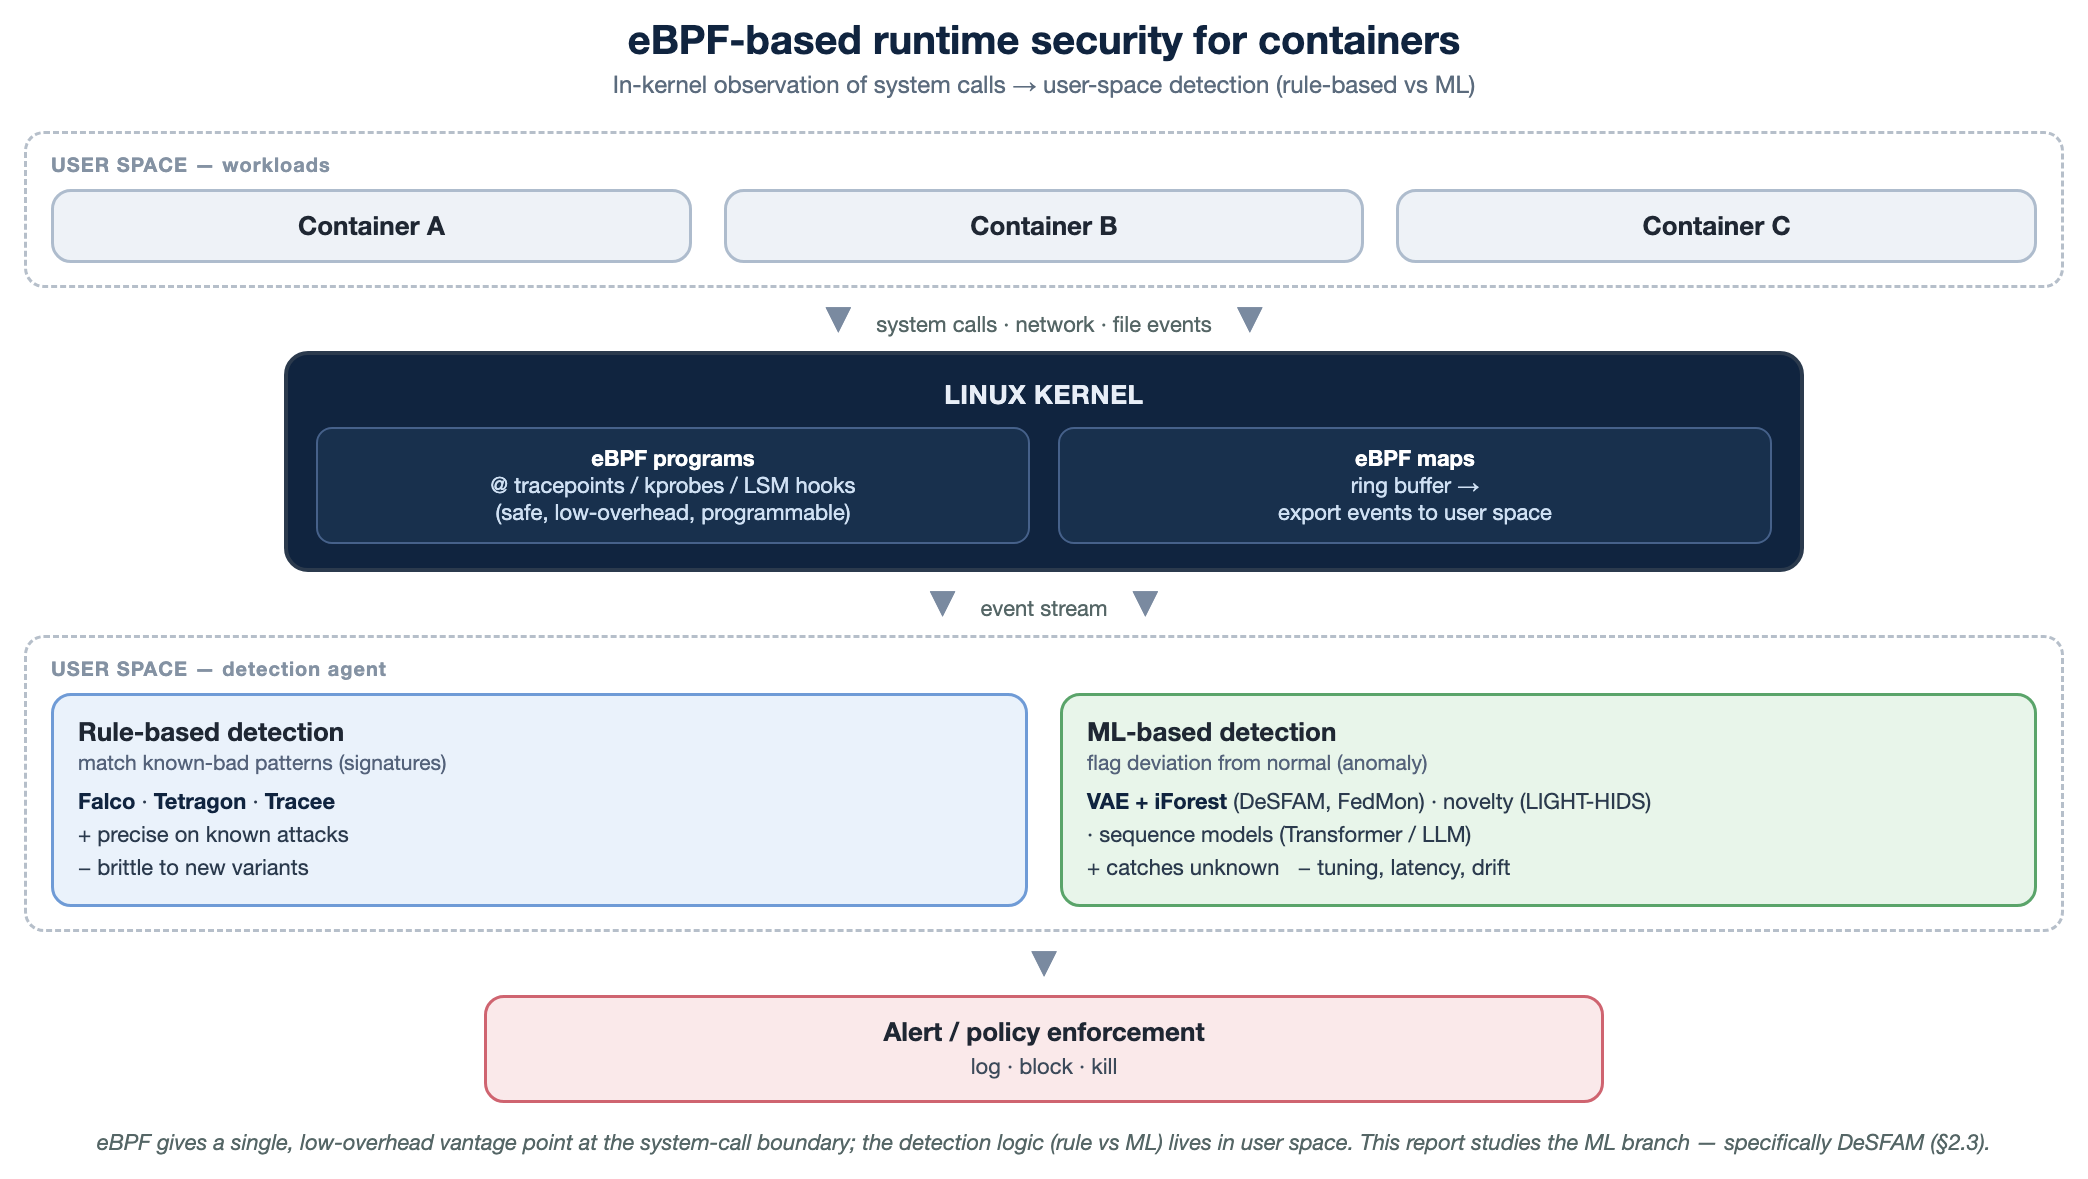
\includegraphics[width=\textwidth]{figures/fig_ebpf_runtime.png}
\caption{Quan sát system call qua eBPF và hai hướng phát hiện (rule-based và ML).}
\label{fig:ebpf}
\end{figure}

\subsection{DeSFAM và cơ chế ngưỡng động}\label{ss:desfam}
DeSFAM~\cite{desfam_original} là khung kết hợp eBPF và học máy cho anomaly detection ở runtime container, được báo cáo lựa chọn làm hệ cơ sở. Thành phần lõi của nó — \textit{SyscallAD} — vận hành theo ba bước. Thứ nhất, mỗi \textit{sliding window} (cửa sổ trượt) các system call được biểu diễn thành một vector đặc trưng gồm tần suất theo nhóm chức năng, đặc trưng thời gian, và mức độ khớp với mẫu hành vi lành tính. Thứ hai, vector này được chấm điểm bất thường bằng một \textit{ensemble} gồm Variational Autoencoder (VAE) và Isolation Forest, cả hai huấn luyện theo chế độ \textit{normal-only} (chỉ trên dữ liệu lành tính) và hợp nhất theo trọng số $0{,}7/0{,}3$. Thứ ba, quyết định cảnh báo dựa trên một \textit{ngưỡng động}: ngưỡng được khởi tạo tại phân vị $99{,}5$ của phân phối điểm bất thường lành tính, rồi cập nhật theo exponential moving average (EMA).

Một điểm mấu chốt cho báo cáo này là \textbf{bản thân DeSFAM mô tả quy tắc cập nhật ngưỡng theo hai cách không nhất quán}. Phần lời quanh công thức (3) viết rằng ngưỡng ``được cập nhật \textit{sau mỗi cửa sổ}'' — đọc theo nghĩa đen là cập nhật \textit{vô điều kiện}. Tuy nhiên, đặc tả hình thức trong \textit{Algorithm 2} của DeSFAM~\cite{desfam_original} lại đặt phép cập nhật trong nhánh \texttt{else}: nếu $A(W_i)>T$ thì gắn cờ (\textit{không} cập nhật ngưỡng), \textit{ngược lại} mới cập nhật $T \leftarrow \max(T_{\min}, \beta T + (1-\beta)A)$. Tức Algorithm 2 \textbf{chỉ cập nhật trên cửa sổ không bị gắn cờ} — cập nhật \textit{có điều kiện}. Sự mơ hồ giữa lời văn (vô điều kiện) và thuật toán (có điều kiện) chính là điểm mà báo cáo khai thác và làm rõ: như sẽ thấy ở Mục~\ref{sec:results}, khác biệt này có \textit{hệ quả an ninh} trực tiếp. Chi tiết hình thức hoá ở Mục~\ref{sec:method}; minh hoạ cơ chế ở Hình~\ref{fig:desfam}. Biến thể federated FedMon~\cite{fedmon2025} kế thừa kiến trúc này và tự thừa nhận hạn chế trước workload \textit{non-IID} (dị thể giữa các tenant) — cho thấy nhiễu đa người thuê là một vấn đề có thật đối với họ DeSFAM; báo cáo này khảo sát chính nhiễu đó dưới \textit{góc độ đối kháng}, chứ không nhằm giải quyết khía cạnh độ chính xác của học liên kết.

\begin{figure}[ht]
\centering
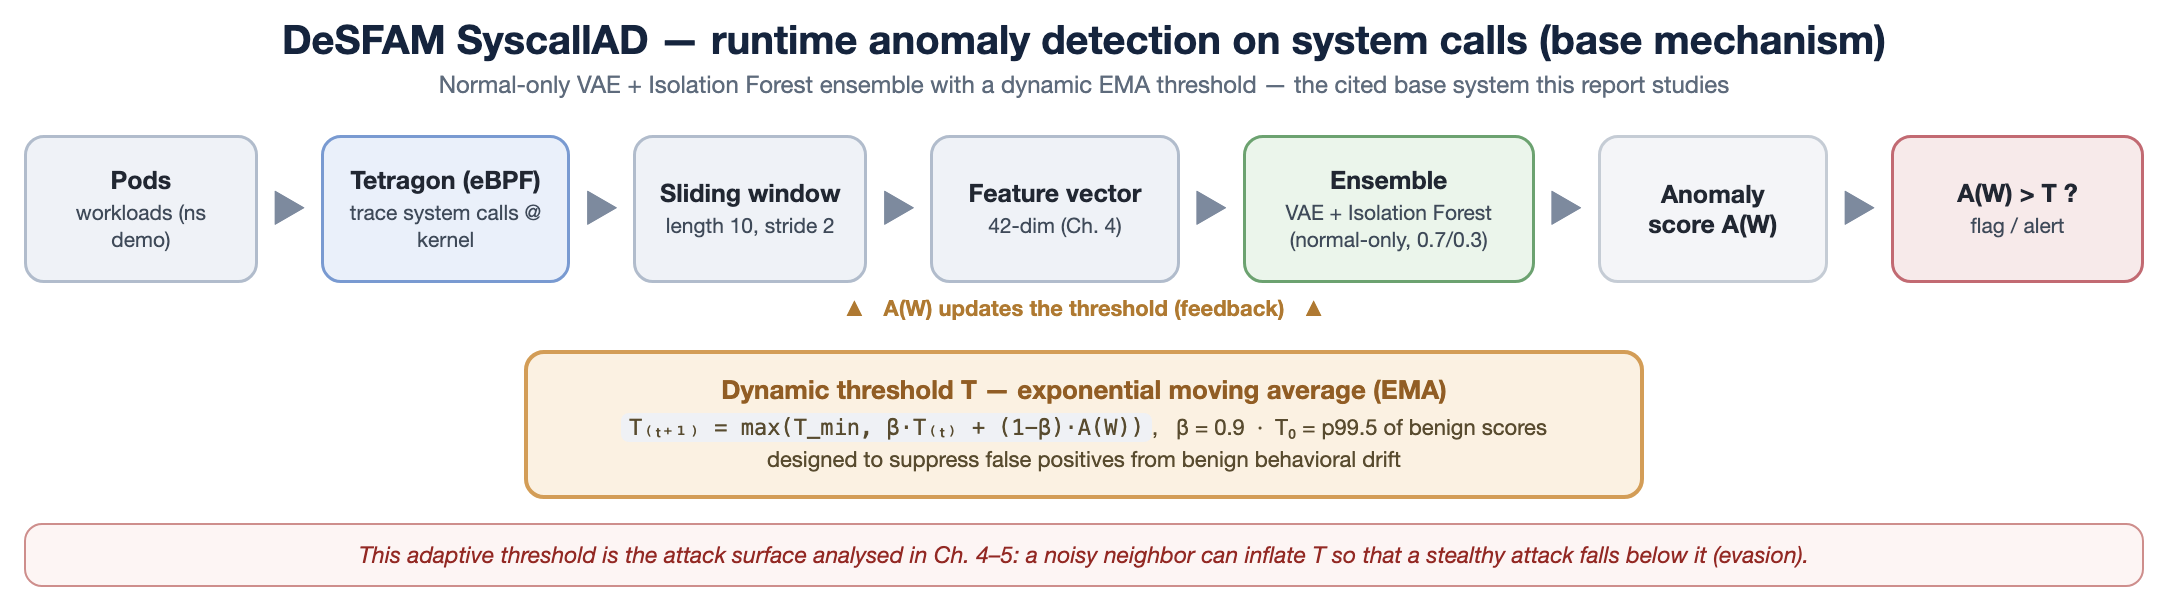
\includegraphics[width=\textwidth]{figures/fig_desfam.png}
\caption{Cơ chế phát hiện của DeSFAM SyscallAD (hệ cơ sở).}
\label{fig:desfam}
\end{figure}

\subsubsection{Vai trò của VAE và Isolation Forest}
Hai mô hình được lựa chọn vì \textit{bổ trợ} cho nhau và đều huấn luyện được theo chế độ \textit{normal-only} — phù hợp với thực tế an ninh, nơi mẫu tấn công hiếm, đa dạng và khó thu thập đầy đủ; do đó việc chỉ học từ hành vi lành tính là khả thi hơn so với học có giám sát cần nhãn tấn công.

\textbf{Variational Autoencoder (VAE)} là một mô hình sinh (generative) học cách nén rồi tái tạo dữ liệu qua một không gian ẩn (latent space) có cấu trúc xác suất. Khi chỉ huấn luyện trên hành vi lành tính, VAE tái tạo tốt các cửa sổ bình thường nhưng tái tạo kém các cửa sổ bất thường; vì vậy \textit{sai số tái tạo} (reconstruction error) lớn được dùng làm điểm bất thường. Ưu điểm là nắm bắt được cấu trúc phi tuyến và phân phối tinh vi của hành vi bình thường; hạn chế là nhạy với tính đại diện của dữ liệu huấn luyện và có thể gặp posterior collapse.

\textbf{Isolation Forest} là một tập hợp cây phân tách ngẫu nhiên: điểm bất thường thường bị \textit{cô lập} chỉ sau vài bước chia, nên độ dài đường đi (path length) ngắn tương ứng với mức bất thường cao. Ưu điểm là nhẹ, không giả định phân phối dữ liệu, ổn định và hiệu quả trên không gian nhiều chiều; hạn chế là chỉ phản ánh mức ngoại lai \textit{toàn cục}, kém tinh tế hơn VAE trước các sai lệch cục bộ.

\textbf{Vì sao kết hợp (ensemble $0{,}7/0{,}3$).} VAE mạnh ở việc mô hình hoá manifold của dữ liệu bình thường nhưng kém ổn định; Isolation Forest thô hơn song bền vững và chi phí thấp. Hợp nhất hai điểm số đã chuẩn hoá theo trọng số $0{,}7$ (VAE) và $0{,}3$ (Isolation Forest) giúp giảm điểm yếu của từng mô hình và cho điểm bất thường ổn định hơn so với khi dùng riêng lẻ. Trọng số $\alpha=0{,}7$ không phải lựa chọn tuỳ ý: nhóm tác giả DeSFAM xác định nó qua phân tích độ nhạy trên $\alpha\in\{0{,}0;\,0{,}25;\,0{,}5;\,0{,}7;\,0{,}85;\,1{,}0\}$, với F1 và AUC đạt đỉnh tại $\alpha=0{,}7$~\cite{desfam_original}.

Bảng~\ref{tab:related} định vị DeSFAM cùng các hướng phát hiện liên quan.

\begin{table}[ht]
\caption{So sánh các hướng phát hiện trên cloud/K8s.}
\label{tab:related}
\centering
\renewcommand{\arraystretch}{1.35}
\begin{tabular}{@{}p{2.9cm}p{3.4cm}C{1.6cm}C{1.7cm}C{1.9cm}@{}}
\toprule
Công trình & Phương pháp & Ngưỡng động & Đa người thuê & Đánh giá đối kháng \\
\midrule
DeSFAM~\cite{desfam_original}             & VAE + iForest          & \yes\,(EMA) & \yes$^\dagger$ & \no \\
FedMon~\cite{fedmon2025}                  & VAE + iForest (FL)     & \yes\,(EMA) & \yes$^\dagger$ & \no \\
Rule-based~\cite{syairozi2025ebpfcompare} & Falco/Tetragon/Tracee  & \no         & \no            & \no \\
Kotenko~\cite{kotenko2025containerae}     & Autoencoder            & \no         & \no            & \no \\
Báo cáo này                               & VAE + iForest (DeSFAM) & \yes\,(EMA) & \yes           & \yes \\
\bottomrule
\end{tabular}
\par\smallskip{\footnotesize \yes\,= có · \no\,= không · $\dagger$\,= có hỗ trợ nhưng chưa kiểm thử dưới điều kiện thù địch.}
\end{table}

\subsection{Khoảng trống nghiên cứu}\label{ss:gap}
Khảo sát ở các Mục~\ref{ss:hids}--\ref{ss:desfam} làm nổi bật hai khoảng trống nghiên cứu chính:
\begin{enumerate}[leftmargin=1.5cm,label=(\roman*)]
\item \textbf{Tác động của nhiễu đa người thuê.} Ảnh hưởng của workload non-IID giữa các tenant lên độ nhạy của bộ phát hiện chưa được định lượng một cách hệ thống — đúng hạn chế mà FedMon~\cite{fedmon2025} tự thừa nhận.
\item \textbf{Hệ quả an ninh của cập nhật ngưỡng vô điều kiện.} Tác động an ninh khi một bộ phát hiện cập nhật ngưỡng thích nghi \textit{vô điều kiện} — như cách đọc theo nghĩa đen công thức (3) của DeSFAM, trái với Algorithm 2 — chưa được định lượng. Nói rộng hơn, khả năng một kẻ tấn công \textit{chủ động} lợi dụng cơ chế tự cập nhật ngưỡng còn ít được khảo sát hệ thống trong runtime container security; mọi đánh giá thuộc họ DeSFAM (Bảng~\ref{tab:related}) đều thực hiện trong điều kiện không thù địch.
\end{enumerate}
Báo cáo tập trung lấp hai khoảng trống này (RQ2); việc tái lập và đánh giá năng lực bộ phát hiện (RQ1) — bao gồm cả phân tích tách theo từng loại tấn công — cung cấp nền tảng cần thiết để khảo sát chúng.
